\PassOptionsToPackage{hidelinks}{hyperref}


\documentclass[man]{apa7}
\usepackage{orcidlink} % Include this for ORCID links


\usepackage{graphicx}
% Define a custom command for including graphics with a max size
\newcommand{\includegraphicsmax}[2][]{%
	\includegraphics[width=\textwidth,height=0.25\textheight,keepaspectratio,#1]{#2}%
}


% Define parameters for subfigure size and vertical space
\newcommand{\subfigwidth}{0.2\textwidth}
\newcommand{\subfigvspace}{0.1em}

\usepackage{subcaption}
\usepackage{tabularx}
\usepackage{floatrow}
\usepackage[T1]{fontenc}
\usepackage[utf8]{inputenc}
\usepackage[spanish]{babel}

\usepackage{textgreek}      % Para usar caracteres griegos en el texto

\usepackage{booktabs}
\usepackage{array}

\usepackage{subcaption}


\usepackage{csquotes}
\usepackage[style=apa,sortcites=true,sorting=nyt,backend=biber]{biblatex}
\DeclareLanguageMapping{american}{american-apa}
\addbibresource{camila.tesis.ufm.bib}

\usepackage{microtype}

\title{Patrones Dietéticos y Síntomas Depresivos en Mujeres Jóvenes Guatemaltecas: Un Análisis de Correlaciones Específicas}
\shorttitle{Dieta y Síntomas Depresivos en Mujeres Guatemaltecas}

\author{
	\href{https://orcid.org/0009-0008-9550-9083}{Dra. Camila Heredia \orcidlink{0009-0008-9550-9083}} 
    y 
    \href{https://orcid.org/0009-0001-2531-6058}{Licda. María Andrée Neumann \orcidlink{0009-0001-2531-6058}}
	}


\authorsaffiliations{Escuela de Postgrado, Universidad Francisco Marroquín}

\leftheader{Heredia, Neumann}

\abstract{Este estudio examina la relación entre marcadores inflamatorios, dieta y
	depresión en mujeres jóvenes guatemaltecas. Utilizando un diseño
	cuantitativo, no experimental y transversal correlacional, se analizó
	una muestra de $30$ participantes mediante la Escala de Depresión de Beck,
	un cuestionario dietético y análisis de sangre para PCR y VS. Los
	resultados revelaron correlaciones significativas entre patrones
	dietéticos y síntomas depresivos. Se encontró una fuerte asociación
	negativa entre el consumo de frutas y síntomas como la pérdida de placer
	$(r = -0.49, p = 0.006)$ y pensamientos suicidas $(r = -0.48, p = 0.007)$.
	El consumo de alimentos procesados se correlacionó positivamente con
	síntomas como pesimismo y pérdida de interés. Aunque no se encontraron
	correlaciones directas entre dieta y marcadores inflamatorios, los
	hallazgos sugieren un posible efecto protector de una dieta rica en
	frutas contra la depresión. El estudio destaca la importancia de
	considerar intervenciones dietéticas en la prevención y tratamiento de
	la depresión en mujeres jóvenes.}

\keywords{Palabras clave: VS, PCR, Beck, ánimo, nutrición}

\authornote{
	Este trabajo se presenta como parte del curso de Metodología de la
	Investigación I impartido por la profesora Regina Fernández Morales
	durante el cuarto ciclo del año 2023 en UFM. El anteproyecto no presenta
	ningún conflicto de interés y el contenido es original en cuanto a la
	revisión de literatura, objetivos y metodología planteados en el mismo.

	La comunicación con las autoras debe realizarse a cualquiera de los
	siguientes correos:
	\href{mailto:camilah@ufm.edu}{\nolinkurl{camilah@ufm.edu}} o
	\href{mailto:mneumann@ufm.edu}{\nolinkurl{mneumann@ufm.edu}}
}

\usepackage{times}

\begin{document}
	\maketitle

	%	\tableofcontents


	\section{Marco contextual}\label{marco-contextual}

	La investigación se llevó a cabo en mujeres jóvenes en la Ciudad de
	Guatemala. La elección de tomar muestras en las clínicas Salud UFM y
	procesarlas en LABOCLIP se basó en la facilidad de acceso y la
	disposición de estas instituciones para participar en el estudio. La
	clínica Salud UFM, siendo una institución que colabora en la toma de
	muestras para investigaciones de sus estudiantes, y LABOCLIP, un
	laboratorio conocido por su disposición a trabajar con la comunidad
	académica, brindaron un entorno propicio para la realización de esta
	investigación.\\

	El estudio que se realizó tiene relevancia actual destacada dado el
	creciente aumento en la prevalencia de la depresión a nivel global. La
	depresión es una enfermedad frecuente en todo el mundo, y se calcula que
	afecta a más de 300 millones de personas. El 7 de abril del 2017, con
	ocasión del Día Mundial de la Salud, la OMS puso en acción una campaña
	anual titulada: ``Hablemos de depresión''. Mostrando así la gran
	preocupación que este tema genera. \parencite{Toshi2022}.\\

	Asimismo, los resultados de esta investigación podrían contribuir
	significativamente a la prevención y al tratamiento de las
	comorbilidades relacionadas con la inflamación crónica, en caso de que
	se confirmara una asociación positiva. En el escenario contrario, si se
	encontrara una asociación negativa o no significativa, los hallazgos aún
	serían valiosos para orientar investigaciones futuras en esta área.

	Aunque estudios similares se han llevado a cabo en distintas
	ubicaciones, carecen de investigaciones parecidas en la población
	guatemalteca en particular. En general, Guatemala ha sido un país en que
	la investigación sobre la depresión ha estado menos presente en
	comparación con otras regiones y es por esto la suma importancia del
	presente estudio.\\

	La depresión es una afección altamente comórbida, lo que significa que a
	menudo se presenta junto con otras enfermedades que están relacionadas
	con la inflamación crónica. Comprender la relación entre la inflamación
	y la depresión podría ayudar a mejorar el manejo de estas condiciones
	médicas comórbidas. Una de las enfermedades comórbidas que se puede
	mencionar es la enfermedad autoinmune. \parencite{Bloch1983}


	\subsection{Marco conceptual}
	La inflamación puede definirse como una respuesta local al daño celular,
	que se caracteriza por aumento del flujo sanguíneo, vasodilatación
	capilar, infiltración de leucocitos y la producción local de mediadores
	de inflamación por parte del huésped. La inflamación es parte de la
	respuesta y es necesario el retorno a la homeostasis luego de daño
	producido por un agente infeccioso, daño físico o estrés metabólico
	\parencite{GarciaCasal2014}.\\

	El proceso de inflamación es una respuesta adaptativa del cuerpo para
	indicar que está en peligro, que necesita atención. El proceso de
	inflamación puede ser entendido como una respuesta biológica altamente
	orquestada. Involucra una serie de eventos a nivel celular y molecular
	que incluyen la liberación de citocinas proinflamatorias, la activación
	de células inmunitarias, y la regulación de mediadores inflamatorios
	como las prostaglandinas y el óxido nítrico \parencite{Stankov2012}.\\

	Además, la inflamación puede clasificarse en dos tipos principales:
	inflamación aguda e inflamación crónica. La inflamación aguda es una
	respuesta rápida y transitoria del cuerpo a una lesión o infección. Este
	tipo de inflamación ayuda a eliminar la causa subyacente y promover la
	curación. Por otro lado, la inflamación crónica es de larga duración y
	puede contribuir al desarrollo de enfermedades crónicas como la artritis
	reumatoide, la enfermedad cardiovascular, Alzheimer, cáncer y diabetes
	tipo 2 \parencite{Osimo2019}.\\

	La nutrición desempeña un papel fundamental en la regulación de la
	inflamación. Algunos nutrientes, como los antioxidantes presentes en
	frutas y verduras; así como los ácidos grasos omega-3 que se encuentran
	en el pescado, tienen propiedades antiinflamatorias. Una dieta
	equilibrada y rica en estos nutrientes puede ayudar a controlar la
	inflamación y prevenir enfermedades relacionadas con la misma.

	Asimismo, el estrés es un factor que puede influir en la inflamación. El
	estrés crónico puede activar el sistema inmunológico y desencadenar una
	respuesta inflamatoria en el cuerpo, lo que a su vez puede tener un
	impacto negativo en la salud a largo plazo. El manejo correcto del
	estrés puede ser una herramienta efectiva para reducir la inflamación
	crónica si es esta la causa subyacente.

	Entre los procesos de inflamación se encuentra el dolor, que a pesar de
	ser un aspecto negativo; es importante destacar que su presencia en
	nuestra vida es la relación de supervivencia y bienestar. Experimentar
	el dolor es señal de advertencia de que algo está mal en el organismo,
	haciendo que nos movilicemos en busca de una solución. El dolor es una
	sensación desagradable que ocurre en diferentes grados de intensidad,
	como consecuencia de una lesión, una enfermedad o un trastorno emocional
	\parencite{Farlex2023}.


	La Asociación Internacional para el Estudio del Dolor (IASP) define el dolor como ``una experiencia sensorial o emocional desagradable, asociada con un daño actual o potencial en los tejidos, que puede describirse en términos de dicho daño'' \parencite{PainTermsList1979}.


	Existen factores nutricionales que pueden afectar o modular el sistema
	inmunitario. Entre ellos se incluyen la ingesta total de calorías. Las
	investigaciones sugieren que la alteración o modulación de la respuesta
	inmunitaria a través de la dieta puede ser útil para prevenir
	inflamaciones \parencite{GarciaCasal2014}.\\

	En los últimos años, han estudiado el eje PINE
	(psicoinmunoneuroendocrinología); en donde demuestra que todos los
	sistemas del cuerpo humano están relacionados y conectados entre sí. Por
	eso mismo, la importancia del estudio del ser humano integralmente. Se
	estudia tanto lo fisiológico como lo mental \parencite{Osimo2019}.\\

	Además, ha habido una acumulación de revisión sistemática
	que sugiere una conexión entre la inflamación y la depresión. La
	inflamación crónica podría desempeñar un papel en la patogénesis de la
	depresión, y la depresión podría causar más inflamación. La palabra
	``depresión'' se utiliza a menudo para describir muchas cosas
	diferentes. Puede definir un estado de ánimo fugaz, o tal vez una
	apariencia física externa de tristeza, o para otros, un trastorno
	clínico diagnosticable. Cada año, millones de adultos sufren depresión
	clínicamente diagnosticada, un trastorno del estado de ánimo que a
	menudo afecta el funcionamiento personal, vocacional, social y de salud
	\parencite{APA2014}.

	\subsection{Estado del arte}

	El estudio de la relación entre la inflamación, dieta y depresión ha
	sido de creciente interés en la última década, aún cuando sigue siendo un área en
	desarrollo. La conexión entre la salud mental y física ha sido una
	preocupación constante en la medicina y la psicología, y más
	recientemente, el papel de la dieta y la inflamación ha emergido como un
	potencial mediador en esta relación.

	El fenómeno inflamatorio ha capturado la atención de la comunidad
	científica debido a su vinculación con diversas enfermedades crónicas.
	Aun cuando la inflamación puede originarse por múltiples causas, como
	infecciones o lesiones, recientemente se ha puesto énfasis en investigar
	el impacto de la dieta como potencial agente proinflamatorio. Esta
	preocupación surge porque una inflamación crónica puede elevar el riesgo
	de condiciones como resistencia a la insulina, diabetes, síndrome
	metabólico y enfermedades cardiovasculares. Por ende, entender y modular
	la inflamación a través de la dieta puede ser clave en la prevención y
	manejo de tales enfermedades \parencites{daneshLowGradeInflammation2000}{ridkerHighsensitivityCreactiveProtein2004}{salas-salvadoConjugatedLinoleicAcid2006}.

	Algunos nutrientes tendrían capacidad antiinflamatoria, mientras que
	otros serían proinflamatorios. Es por eso la importancia conocer cuáles
	son los nutrientes capaces de modular la inflamación y en qué cantidad
	se deben administrar \parencite{giuglianoMetabolicCardiovascularEffects1997}.

	Es esencial mencionar que la mayoría de los estudios emplearon regresión
	lineal múltiple para sus análisis y se ajustaron por factores como
	género, edad, estatus socioeconómico, índice de masa corporal (IMC),
	entre otros. Estos hallazgos refuerzan la relevancia de la dieta en
	relación con marcadores inflamatorios y cardiometabólicos en poblaciones
	jóvenes \parencite{cotaCardiometabolicRiskHealth2021}.

	En un meta-análisis, se revisaron $1,545$ estudios, de los cuales $37$
	cumplieron con los criterios de inclusión para investigar la relación
	entre inflamación y depresión. De estos, se determinó que el $27\%$ de los
	$11,813$ pacientes con depresión analizados mostraron inflamación de bajo
	grado. A pesar de la heterogeneidad entre estudios, los análisis de
	sensibilidad confirmaron una prevalencia similar. Notablemente, al
	comparar pacientes con depresión con controles no deprimidos, aquellos
	con depresión tuvieron 1.46 veces mayor probabilidad de presentar
	inflamación de bajo grado. Estos hallazgos sugieren una relevancia
	significativa de la inflamación en un amplio segmento de pacientes con
	depresión \parencite{Osimo2019}.

	De acuerdo a \parencite{Farre2020}, la alimentación es esencial no sólo
	para nuestra supervivencia y crecimiento, sino también para mantener la
	homeostasis de diferentes componentes de la barrera mucosa. Las
	investigaciones han evidenciado que los nutrientes tienen roles
	cruciales en: (1) mantener el epitelio intestinal, favoreciendo el
	crecimiento celular, su homeostasis y funciones; (2) regular la función
	de la barrera epitelial intestinal; (3) modular la inmunidad intestinal;
	y sorprendentemente, (4) la suplementación nutricional podría mejorar
	las anomalías mucosas presentes en pacientes con trastornos
	gastrointestinales.\\

	Este panorama refuerza la relevancia de los nutrientes en la homeostasis
	de la barrera mucosa y el mantenimiento de la fisiología normal del
	intestino. Se requieren más ensayos clínicos bien diseñados para
	confirmar la posibilidad de la suplementación nutricional como
	tratamiento para pacientes con disfunción de la barrera mucosa,
	incluyendo a aquellos con enfermedades como enfermedad celíaca,
	sensibilidad al gluten no celíaca, síndrome del intestino irritable y
	dispepsia funcional \parencite{Farre2020}.

	Con el apoyo del Instituto Nacional del Corazón, los Pulmones y la
	Sangre (NHLBI, por sus siglas en inglés), se evaluó la capacidad de los
	marcadores inflamatorios y lipídicos para predecir el riesgo de eventos
	cardiovasculares en un estudio de casos y controles de 366 mujeres
	aparentemente sanas inscritas en el Estudio de Salud de la Mujer. De los
	12 marcadores evaluados, la PCR era la variable más fuerte para predecir
	las inflamaciones \parencite{ridkerHighsensitivityCreactiveProtein2004}.

	A continuación, se detallan investigaciones que han explorado esta
	conexión y sus conclusiones. En una revisión sistemática, la interacción
	entre inflamación y depresión ha sido explorada en 109 estudios, cuya
	calidad en su mayoría se catalogó de moderada a alta \parencite{Toenders2022}.\\

	Al examinar medidas dimensionales de síntomas depresivos, la mayoría de
	estudios no encontraron una correlación significativa entre la severidad
	de la depresión y marcadores inflamatorios clave como $IL-1\textbeta$, IL-6 y CRP
	en jóvenes saludables, sugiriendo que niveles clínicos de depresión
	podrían ser necesarios para observar una disfunción inflamatoria
	\parencite{Toenders2022}.\\

	Desde una perspectiva longitudinal, se ha observado variabilidad en las respuestas inflamatorias tras diferentes intervenciones terapéuticas. Por ejemplo, un estudio sobre la terapia cognitivo-conductual (TCC) para el insomnio en pacientes con osteoartritis de rodilla examinó sus efectos en la inflamación sistémica \parencite{munPreliminaryExaminationEffects2024}. En el caso de pacientes con cáncer de mama, una investigación evaluó el impacto de formas breves de manejo del estrés, incluyendo TCC, en los niveles de S100A8/A9 asociados con RAGE, un marcador relacionado con la inflamación y el desarrollo tumoral \parencite{taubEffectsRandomizedTrial2019}. Además, en pacientes con insuficiencia cardíaca, se analizaron los efectos de la TCC para el insomnio sobre la función autonómica y los marcadores inflamatorios \parencite{redekerEffectsCognitiveBehavioral2020}. Estos estudios sugieren que los efectos de las intervenciones psicológicas en los marcadores inflamatorios no son uniformes y pueden variar según la condición tratada y los biomarcadores específicos medidos. Las divergencias observadas podrían atribuirse a diferencias en los protocolos de tratamiento, las poblaciones estudiadas o las complejas interacciones entre los diversos componentes del sistema inmunológico e inflamatorio.

	\subsection{Planteamiento del problema}

	La relación entre inflamación y depresión, como se ha mencionado anteriormente, ha sido objeto de múltiples
	investigaciones a nivel global, habiendo evidencia robusta que vincula
	marcadores inflamatorios y episodios depresivos en diversas poblaciones.
	Sin embargo, la mayoría de estos estudios se han centrado en poblaciones
	específicas, dejando a muchas regiones, como es el caso de Centroamérica, con una
	notable insuficiencia de datos en este ámbito.\\

	Guatemala, a pesar de tener una población con rasgos sociodemográficos,
	genéticos y ambientales únicos, carece de investigaciones que aborden la
	interacción entre inflamación y depresión. Esta brecha de conocimiento
	se agrava al considerar que no solo no se ha explorado la relación entre
	inflamación y depresión per sé, sino que tampoco se ha analizado cómo
	factores socioeconómicos y demográficos guatemaltecos modulan dicha
	relación. En el contexto guatemalteco, donde la diversidad genética y la
	variabilidad en factores ambientales y socioeconómicos es significativa,
	es imperativo llenar esta laguna informativa para ofrecer intervenciones
	y tratamientos más contextualizados.

	La presente investigación busca responder a la imperante pregunta: ¿Cómo
	se relacionan los marcadores inflamatorios con la severidad de los
	síntomas depresivos y los hábitos alimenticios en la población de
	mujeres jóvenes guatemaltecas?

	\section{Objetivos}\label{objetivos}

	\subsection{Objetivo General}\label{objetivo-general}

	Analizar la relación entre los marcadores inflamatorios, la severidad de
	los síntomas depresivos y hábitos alimenticios en la población de
	mujeres jóvenes guatemaltecas.

	\subsection{Objetivos Específicos}\label{objetivos-especuxedficos}

	\begin{enumerate}
		\item Identificar y cuantificar los principales marcadores inflamatorios presentes en mujeres de jóvenes guatemaltecas.
		\item Identificar los síntomas depresivos por medio de la escala de Beck.
		\item Determinar o caracterizar los hábitos alimentarios de las mujeres de jóvenes guatemaltecas por medio de un cuestionario.
		\item Establecer el grado de correlación entre la presencia de determinados marcadores inflamatorios y hábitos alimenticios.
		\item Describir la distribución de síntomas depresivos en la población de mujeres de jóvenes guatemaltecas en función de su nivel de inflamación.
	\end{enumerate}


	\section{Materiales y métodos}\label{materiales-y-muxe9todos}

	\subsection{Diseño investigación}\label{diseuxf1o-investigaciuxf3n}

	El diseño de esta investigación fue cuantitativo, no experimental y
	transversal correlacional. Este enfoque se eligió cuidadosamente para
	estudiar de manera objetiva la correlación entre la dieta y el estado
	anímico de la muestra contando con marcadores inflamatorios
	específicos.\\

	\subsubsection{Enfoque} En este estudio, el enfoque cuantitativo se empleó para
	medir y analizar las variables de manera numérica y estadística. Se
	estuvo particularmente interesado en medir cómo la variación en los
	marcadores inflamatorios fue descrita a partir de la(s) variable(s)
	independiente(s), es decir, cómo la dieta y el estado anímico pudieron
	influir en los niveles de marcadores inflamatorios como la proteína C
	reactiva y la eritrosedimentación. Este enfoque cuantitativo permitió una
	evaluación objetiva y precisa (especialmente en el coeficiente
	\emph{$R^2$}) de las relaciones entre estas variables, facilitando así
	conclusiones basadas en datos.\\

	\subsubsection{Alcance}
	El alcance de esta investigación fue correlacional.
	Se buscó entender cómo la dieta y la inflamación en el cuerpo estaban relacionadas
	con el estado anímico. Al analizar estas correlaciones, se
	esperó descubrir si existían asociaciones estadísticamente significativas
	que podrían sugerir (más no probar) una relación causal o influencia
	entre los factores.

	\subsubsection{Técnicas}
	Para obtener datos confiables y precisos, se empleó una combinación de técnicas. Se realizó un muestreo de sangre en mujeres jóvenes de la Ciudad de Guatemala. A través de este muestreo, se midieron los marcadores inflamatorios mencionados: proteína C reactiva y eritrosedimentación. Además, se utilizó la escala de depresión de Beck, el cual es un instrumento validado y confiable para medir el estado anímico.

	\subsubsection{Cuestionario de dieta}
	Complementariamente, para poder recopilar información detallada sobre la dieta de las participantes, se aplicó un cuestionario diseñado específicamente para este estudio. Este enfoque de técnicas combinadas permitió analizar las relaciones entre inflamación, estado anímico y dieta de manera holística y sistemática.



	\subsection{Instrumentos}\label{instrumentos}

	Se empleó una combinación de instrumentos
	meticulosamente seleccionados para evaluar con precisión las
	interrelaciones entre dieta, estado anímico y marcadores inflamatorios
	en mujeres jóvenes de la Ciudad de Guatemala.\\

	\subsubsection{Cuestionario de Hábitos Dietéticos}
	Este cuestionario fue diseñado para obtener información detallada y relevante sobre el consumo de alimentos y además sobre los patrones dietéticos de las participantes. Este cuestionario, siguiendo las mejores prácticas en la creación de cuestionarios, incluyó preguntas cuidadosamente formuladas para garantizar la precisión y relevancia de los datos escogidos.\\

	\subsubsection{Escala de Depresión de Beck}
	Este instrumento validado y ampliamente reconocido y utilizado, fue aplicado para medir la severidad de los síntomas depresivos de las participantes. Esta escala facilitó una evaluación cuantitativa y comparativa de los estados anímicos, permitiendo así correlacionar estos datos con los hábitos dietéticos y marcadores inflamatorios. Este cuestionario consta de 21 grupos de afirmaciones.\\

	El puntaje total se obtuvo de la suma de cada uno de los reactivos, siendo 0 el puntaje mínimo y 63 el máximo. Las normas de calificación en población mexicana son, a saber: de 0 a 5 puntos, ansiedad mínima; de 6 a 15, ansiedad leve; de 16 a 30 puntos, ansiedad moderada, y de 31 a 63, ansiedad severa \parencite{beckDepressionCausesTreatment2009}.\\

	\subsubsection{Pruebas de Laboratorio para Marcadores Inflamatorios}
	Como parte del proceso de muestreo, se llevaron a cabo análisis clínicos para identificar y cuantificar los marcadores inflamatorios mencionados con anterioridad: proteína C reactiva y la eritrosedimentación. Estas pruebas generaron una base objetiva de datos clínicos que se utilizó en conjunto con los demás instrumentos para permitir un análisis integral de las interacciones entre las distintas variables.

	\subsection{Muestra y población}\label{muestra-y-poblaciuxf3n}

	La población de la presente investigación estuvo conformada por una
	muestra homogénea de 30 mujeres jóvenes, residentes de la Ciudad de
	Guatemala. Se eligieron 30 mujeres, ya que se asumió que con esa muestra
	se podría lograr normalidad \parencite{Hernandez2018}. Las
	participantes fueron seleccionadas para proporcionar una perspectiva
	representativa sobre las interacciones entre dieta, estado anímico y
	marcadores inflamatorios.

	Para el estudio se tomaron en consideración los siguientes criterios de
	inclusión:
	\begin{enumerate}
		\item Mujeres
		\item de 25 a 30 años
		\item Vivir en la Ciudad de Guatemala
		\item Disposición a participar en el estudio
	\end{enumerate}


	Asimismo, dentro de los criterios de exclusión se identificaron los
	siguientes: a) Mujeres con enfermedad inflamatoria b) mujeres con
	enfermedad autoinmune c) mujeres embarazadas, para evitar cualquier
	influencia de estas condiciones en los marcadores inflamatorios.
	Aclarando estas exclusiones, se advirtió a las participantes que, de no
	cumplirse las exclusiones por parte de ellas, las investigadoras no se
	hacían responsables, ya que firmaron y leyeron el consentimiento
	informado. Esta metodología de selección de muestra y población
	garantizó que la investigación fuera precisa, relevante y replicable.

	\subsection{Selección y definición de variables}\label{selecciuxf3n-y-definiciuxf3n-de-variables}

	En este estudio, se seleccionaron variables que abarcaron aspectos
	bioquímicos, psicológicos y nutricionales. Integrando así, medidas tanto
	cuantitativas como cualitativas con el fin de tener un análisis integral
	y comprensivo.\\

	\subsubsection{Escala de Beck para la Depresión}
	Esta es una medida ordinal que evaluó la severidad de los síntomas depresivos. La escala es una herramienta psicométrica validada y recomendada, y su inclusión permitió cuantificar el estado anímico de las participantes de una manera estandarizada y confiable.

	\subsubsection{Cuestionario de Dieta}
	Se trata de una variable categórica diseñada para evaluar los hábitos dietéticos de las participantes al igual que la calidad. Este cuestionario ayudó a capturar la información de manera detallada sobre el consumo de alimentos y patrones dietéticos, lo cual fue de suma importancia para investigar la relación entre la dieta y los marcadores inflamatorios.



	\section{Hipótesis}\label{hipuxf3tesis}

	Existe una relación bidireccional significativa entre la dieta y la
	depresión, la cual influye en los niveles de marcadores inflamatorios en
	el organismo.

	Basándonos en una revisión comprehensiva de la literatura y en la
	comprensión de las interacciones entre dieta, estado anímico y
	respuestas inflamatorias, se propone la siguiente hipótesis: ``Existe una
	relación bidireccional estadísticamente significativa entre la dieta y
	la depresión, la cual influye en los niveles de marcadores inflamatorios
	del organismo''. Esta hipótesis se sustenta en la premisa de que los
	patrones dietéticos en efecto contribuyen a una afectación del estado
	anímico y, a su vez, influye en los procesos inflamatorios del cuerpo,
	siendo bidireccional, el caso viceverso es verdadero. La confirmación o
	refutación de esta hipótesis aportará valiosa información sobre cómo
	estos factores interactúan y se influencian mutuamente.

	\section{Procedimiento para recolección de datos}\label{procedimiento-para-recolecciuxf3n-de-datos}

	Luego de que se autorizó el tema y la metodología por hacer en
	esta presente investigación, fue sumamente necesario realizar una
	revisión detallada de la literatura para avalar la importancia de la
	investigación. Se garantizó que los antecedentes estuvieran actualizados y
	con una alta fiabilidad.

	Se aseguró que el instrumento de la matriz fuera fiable para elegir entre los artículos buscados. Para esto fue necesario nombrar los diferentes criterios de inclusión y de exclusión. Los criterios para la selección de artículos fueron de suma importancia para asegurarse de que fueran específicos y claros. Asimismo, se necesitaron investigaciones de mujeres de jóvenes guatemaltecas con inflamaciones, investigando la dieta y su estado anímico, encontrando instrumentos específicos como escalas para medir el estado de ánimo.

	Se utilizaron los resultados de los artículos que se creyeron
	pertinentes y necesarios para la investigación. Entre dos
	investigadores, encargados de esta investigación, revisaron los datos
	para minimizar sesgos y poder extraer los datos más precisos.

	Los datos de la investigación se agruparon en base a la dieta y la
	escala de estado de ánimo. Se consideró una escala para medir el estado
	anímico y una entrevista para analizar la dieta de cada participante de
	la investigación, utilizándolos en base a la inflamación que se produce
	a consecuencia del análisis mencionado anteriormente.

	\subsection{Análisis estadístico y procesamiento de datos}

	El análisis estadístico y el procesamiento de datos constituyó la
	columna vertebral de esta investigación; debido a que al proporcionar el
	fundamento cuantitativo necesario se pudo evaluar la hipótesis y
	concluir. A continuación se detalla el enfoque metodológico y las
	distintas técnicas estadísticas que se utilizaron para explorar y comprender
	las interrelaciones entre las variables de estudio. A través de un
	proceso riguroso y sistemático, se propuso descubrir patrones,
	tendencias y correlaciones estadísticamente significativas que arrojaron
	luz sobre las complejas dinámicas entre la dieta, el estado anímico y
	los marcadores inflamatorios.

	\subsection{Descripción y Justificación de Métodos y Técnicas de Análisis}\label{descripciuxf3n-y-justificaciuxf3n-de-muxe9todos-y-tuxe9cnicas-de-anuxe1lisis}

	La elección de métodos y técnicas de análisis estadísticos para este
	estudio estuvo guiada por principios estadísticos y se fundamentó en una
	comprensión profunda de la naturaleza de las variables involucradas.
	Dado que el objetivo fue examinar las posibles correlaciones entre
	variables: hábitos dietéticos, estados anímicos y marcadores
	inflamatorios, se emplearon técnicas de correlación y regresión para
	investigar las relaciones entre las variables. La correlación permitió
	determinar la fuerza y dirección de la relación entre dos
	variables, mientras que el análisis de regresión ayudó a
	comprender cómo la variación en la variable dependiente fue descrita a
	partir de las variables independientes.\\

	Además, considerando la naturaleza de los datos recolectados, que
	incluyeron medidas continuas (marcadores inflamatorios) y ordinales
	(escala de Beck), se utilizaron métodos que se ajustaron a estas
	características. Dentro de ellas estuvieron pruebas de normalidad para
	evaluar la distribución de la muestra; paso crucial para seleccionar las
	pruebas estadísticas más apropiadas. Asimismo, se utilizaron análisis de
	varianza cuando fue relevante para poder comparar las medias entre
	diferentes grupos y entender mejor las variaciones en las variables
	de interés.\\

	Este enfoque no solo permitió establecer la existencia de las
	correlaciones sino también explorar la naturaleza y significado de estas
	relaciones, proporcionando una base sólida para interpretaciones y
	conclusiones posteriores.

	\subsection{Procedimientos Estadísticos}\label{procedimientos-estaduxedsticos}

	\subsubsection{Aplicación y Análisis de la Escala de Depresión de Beck}
	Tras aplicar la escala a la muestra, se categorizaron a los participantes basados en grupos según sus puntuaciones: mínima o ninguna depresión, depresión leve,
	moderada y severa. Esta clasificación fue el eje central para los
	análisis siguientes.\\

	\subsubsection{Pruebas de Normalidad}
	Antes de proceder con análisis
	comparativos, como parte de los procesos estadísticos, un paso crucial
	fue analizar la normalidad de la muestra. Para eso se utilizó la
	prueba de \emph{Shapiro-Wilk} implementada en \emph{`SciPy'} para verificar la
	distribución de los datos. De ser una muestra normal se pudo proceder
	con las siguientes pruebas estadísticas.\\

	\subsubsection{Comparaciones Varianza (ANOVA)} Se utilizó un análisis de
	varianza para comparar los niveles de marcadores inflamatorios y
	patrones dietéticos entre los diferentes grupos de depresión. Si se
	identificaron diferencias significativas, se procedió con pruebas
	post-hoc para identificar dónde residían dichas diferencias.\\

	\subsubsection{Correlación y Análisis de Regresión} Se exploró la relación
	entre la severidad de los síntomas depresivos y los hábitos dietéticos,
	así como los niveles de marcadores inflamatorios, utilizando el
	coeficiente de correlación de Pearson y análisis de regresión. Esto permitió
	entender mejor la naturaleza y fuerza de estas relaciones.

	\subsubsection{Visualización y Presentación de Datos}
	Con el apoyo del lenguaje de programación \emph{`Python'} y \emph{`Jupyter Notebook'} para el análisis estadístico y Tableau para la visualización, se presentaron los datos de manera que resaltaran las relaciones clave y los hallazgos importantes, facilitando su interpretación.

	\subsubsection{Interpretación Contextualizada de Resultados}
	Todos los resultados fueron interpretados considerando la confiabilidad y significancia estadística. Las conclusiones se discutieron en el contexto de la literatura existente y las implicaciones prácticas para el contexto científico general y aplicado a la población guatemalteca.

	\subsection{Inclusión de Aspectos Clave en el Análisis}\label{inclusiuxf3n-de-aspectos-clave-en-el-anuxe1lisis}

	En esta investigación, la integridad y exactitud del análisis
	estadístico fueron fundamentales. Por lo tanto, se incorporaron varios
	aspectos clave que garantizaron la calidad y fiabilidad de los
	resultados y conclusiones.\\

	\subsubsection{Verificación de Normalidad de los Datos}
	En cada etapa del análisis se llevaron a cabo pruebas de normalidad, como la prueba
	Shapiro-Wilk para evaluar la distribución de los datos donde fue
	requerido. Esta verificación fue crucial para determinar el grado de
	idoneidad para la elección de pruebas estadísticas dada la normalidad de la
	muestra y así garantizar la validez de las interpretaciones propuestas.

	\subsubsection{Evaluación de la Confiabilidad de las Herramientas de Medición}
	Fue esencial y fundamental validar la confiabilidad de las herramientas utilizadas, como la escala de Depresión de Beck y el Cuestionario Dietético. Esto se realizó mediante el cálculo del coeficiente alfa de Cronbach, dado que una alta confiabilidad aseguró que los datos recolectados fueran consistentes y representativos.

	\subsubsection{Estadísticas Descriptivas de la Muestra}
	Se proporcionaron estadísticas descriptivas sobre la muestra, incluyendo medias, medianas, modas, rangos y desviaciones estándar. Estas estadísticas ofrecieron una visión clara y comprensible de los datos para establecer análisis basados en un fundamento sólido para subsiguientes pruebas estadísticas.

	\subsubsection{Interpretación Contextualizada de Resultados} Todos los
	resultados se interpretaron a la luz de una hermenéutica contextualizada
	basada en la confiabilidad y significancia estadística respectiva.
	Asimismo, se establecieron umbrales claros para la significancia
	estadística, y los hallazgos se discutieron en relación con estos
	criterios. Esto permitió evaluar la fuerza y relevancia de tanto
	los resultados como las conclusiones presentadas. Además, se buscó
	presentar los resultados basados en la literatura existente y
	teorías relevantes en el campo. Esto proporcionó conclusiones
	relevantes al pueblo latinoamericano, especialmente guatemalteco.

	\section{Consideraciones Éticas}\label{consideraciones-uxe9ticas}

	\subsection{Consentimiento Informado}\label{consentimiento-informado}

	Se obtuvo el consentimiento informado de todos los participantes. Para
	conseguirlo, se les proporcionó información detallada sobre los
	objetivos del estudio, los procedimientos, posibles riesgos y los
	beneficios. Asimismo, se aseguró que entendieran que su participación fue
	completamente voluntaria y que tenían el derecho a retirarse del estudio
	en cualquier momento sin consecuencias.

	\subsection{Confidencialidad y Privacidad}\label{confidencialidad-y-privacidad}

	Se mantuvo la confidencialidad y privacidad de toda la información
	recopilada. Los datos personales de los participantes se anonimizaron y se
	mantuvieron confidenciales, asegurando su privacidad y
	protección.

	\subsection{Aprobación de un Comité de Ética}\label{aprobaciuxf3n-de-un-comituxe9-de-uxe9tica}

	El protocolo de investigación fue sometido para su revisión y
	aprobación a un comité de ética, asegurando así que cumpliera con los
	estándares éticos y normas vigentes.

	\subsection{Impacto y Beneficio para los Participantes y la Comunidad}\label{impacto-y-beneficio-para-los-participantes-y-la-comunidad}

	Se evaluó y describió el impacto potencial y los beneficios de la
	investigación tanto para los participantes como para la comunidad
	involucrada. Asimismo, se hizo hincapié en maximizar los beneficios y
	minimizar cualquier riesgo potencial.

	\subsection{Presupuesto}\label{presupuesto}

	\begin{table}[H]
		\centering
		\begin{tabular}{>{\bfseries}l c}
			\toprule
			Ítem & Costo (Q) \\

			\midrule
			Curitas & 30 \\

			Agujas & 150 \\

			Algodón & 20 \\

			Alcohol & 20 \\

			Gasolina & 200 \\

			Luz e internet & 100 \\

			\midrule
			Total & 520 \\

			\bottomrule
		\end{tabular}
		\caption{Presupuesto para el estudio}
		\label{tab:presupuesto}
	\end{table}




	El presupuesto lo cubrirán las investigadoras principales.

	\subsection{Cronograma}\label{cronograma}

	\begin{table}[h!]
		\centering
		\begin{tabular}{@{}ll@{}}
			\toprule
			\textbf{Item}                & \textbf{Detalle}     \\ \midrule
			Fecha de Inicio              & febrero 2024         \\
			Fecha de Finalización        & junio 2024           \\
			Duración                     & 5 meses              \\ \bottomrule
		\end{tabular}
		\caption{Fechas y Duración del Estudio}
		\label{tab:fechas-duracion}
	\end{table}


	\section{Resultados}\label{resultados}

	\subsection{Datos sociodemográficos}

	\begin{figure}[H]
		\centering
		\includegraphicsmax{freq.age.pdf}
		\caption{Frequencia de Edades}
		\label{fig:Figure1}
	\end{figure}


	\begin{table}[H]
		\centering
		\resizebox{0.8\columnwidth}{!}{
			\begin{tabular}{@{}rrrrr@{}}
				\toprule
				\textbf{Estadístico}             & \textbf{Total de Beck} & \textbf{Total de Dieta} & \textbf{VS} & \textbf{PCR} \\ \midrule
				\textbf{N}                       & 30.00                  & 30.00                   & 30.00       & 30.00        \\
				\textbf{Media}                   & 19.00                  & 4.77                    & 10.27       & 2.56         \\
				\textbf{Mediana}                 & 17.00                  & 6.00                    & 9.00        & 1.45         \\
				\textbf{Desviación estándar}     & 9.28                   & 9.58                    & 6.58        & 2.52         \\
				\textbf{Mínimo}                  & 7.00                   & -17.00                  & 1.00        & 0.00         \\
				\textbf{Máximo}                  & 42.00                  & 21.00                   & 26.00       & 7.60         \\
				\textbf{Asimetría}               & 0.97                   & -0.22                   & 0.81        & 0.79         \\
				\textbf{Curtosis}                & 0.14                   & -0.60                   & 0.36        & -0.89        \\
				\textbf{W de Shapiro-Wilk}       & 0.90                   & 0.97                    & 0.93        & 0.83         \\
				\textbf{Valor p de Shapiro-Wilk} & 0.01                   & 0.63                    & 0.06        & 0.00         \\ \bottomrule
			\end{tabular}
		}

		\caption{Estadísticas descriptivas de las variables}

		\label{tab:descriptives}
	\end{table}


	\subsubsection{Total Escala de Beck}
	La puntuación en la escala de Beck muestra una distribución no normal con una tendencia a la derecha. Esto sugiere que hay más individuos con puntuaciones más bajas en depresión, pero con una amplia variabilidad. La desviación estándar alta indica diferencias significativas entre las puntuaciones individuales.

	\subsubsection{Total Cuestionario Dieta}
	La distribución de las puntuaciones de dieta es normal y tiene valores negativos, lo que es permitido por el cuestionario. La mediana es mayor que la media, indicando una ligera tendencia a valores más altos.

	\subsubsection{Velocidad de Eritrosedimentación}
	La puntuación de VS muestra una ligera desviación a la derecha, lo que indica que la mayoría de las observaciones están por debajo de la media, pero hay algunas puntuaciones significativamente altas.

	\subsubsection{Proteína C Reactiva}
	Las puntuaciones de PCR también están sesgadas a la derecha y no siguen una distribución normal. La mediana significativamente más baja que la media sugiere que la mayoría de las observaciones tienen valores bajos de PCR, pero hay algunas observaciones con valores mucho más altos, indicando posibles casos de inflamación aguda en algunos individuos.

\begin{figure}[H]
	\centering
	\begin{subfigure}[b]{\subfigwidth}
		\centering
		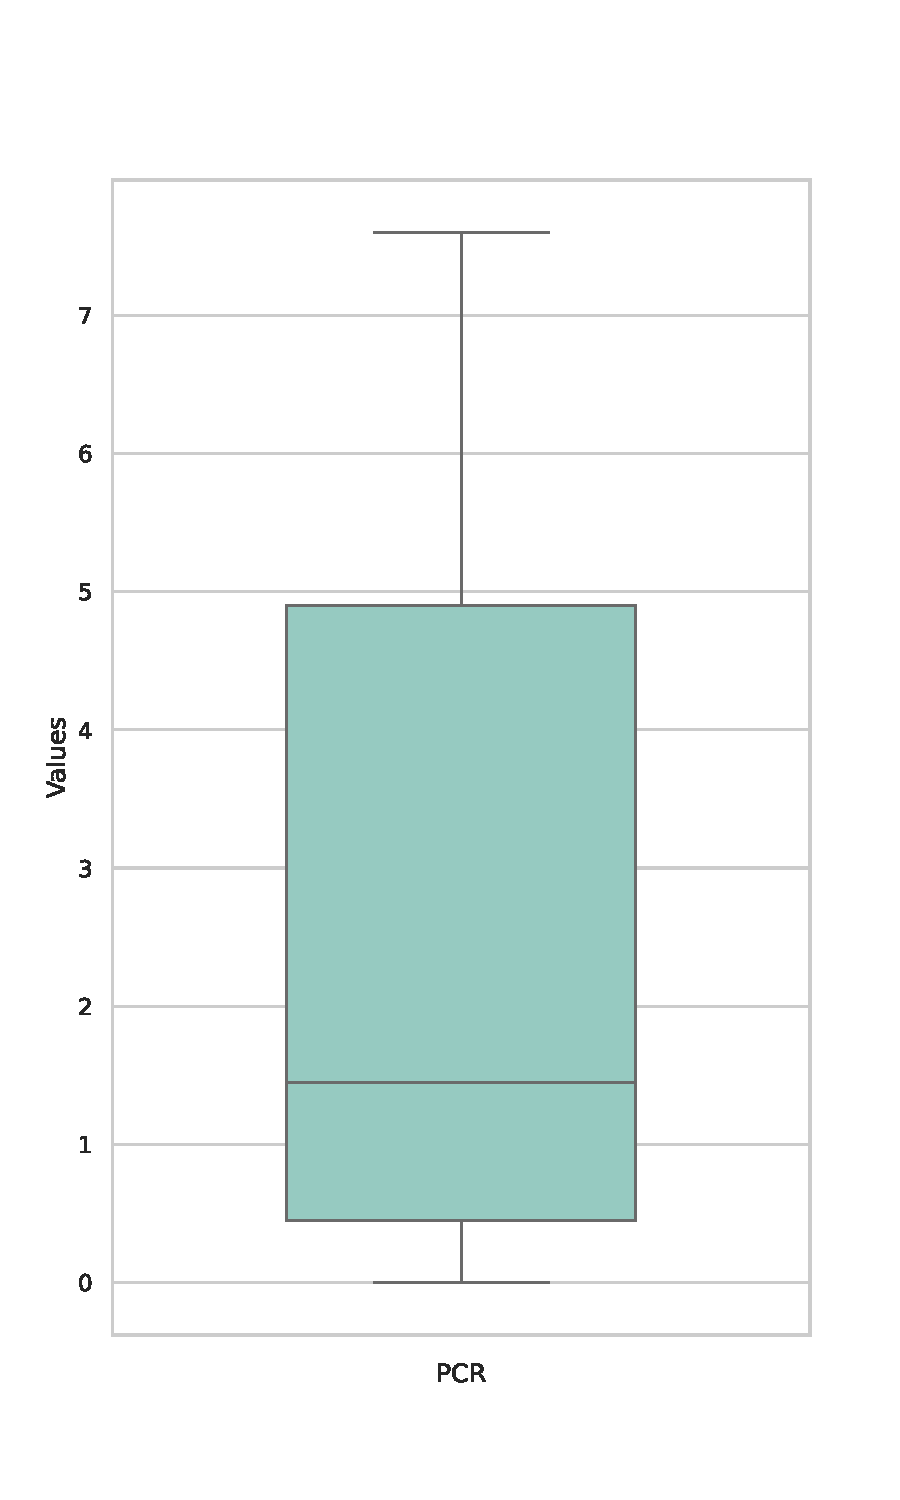
\includegraphics[width=\linewidth]{Box_Plot_of_PCR.pdf}
		\caption{PCR}
		\label{fig:BoxPlotPCR}
	\end{subfigure}
	\hspace{0.5em}
	\begin{subfigure}[b]{\subfigwidth}
		\centering
		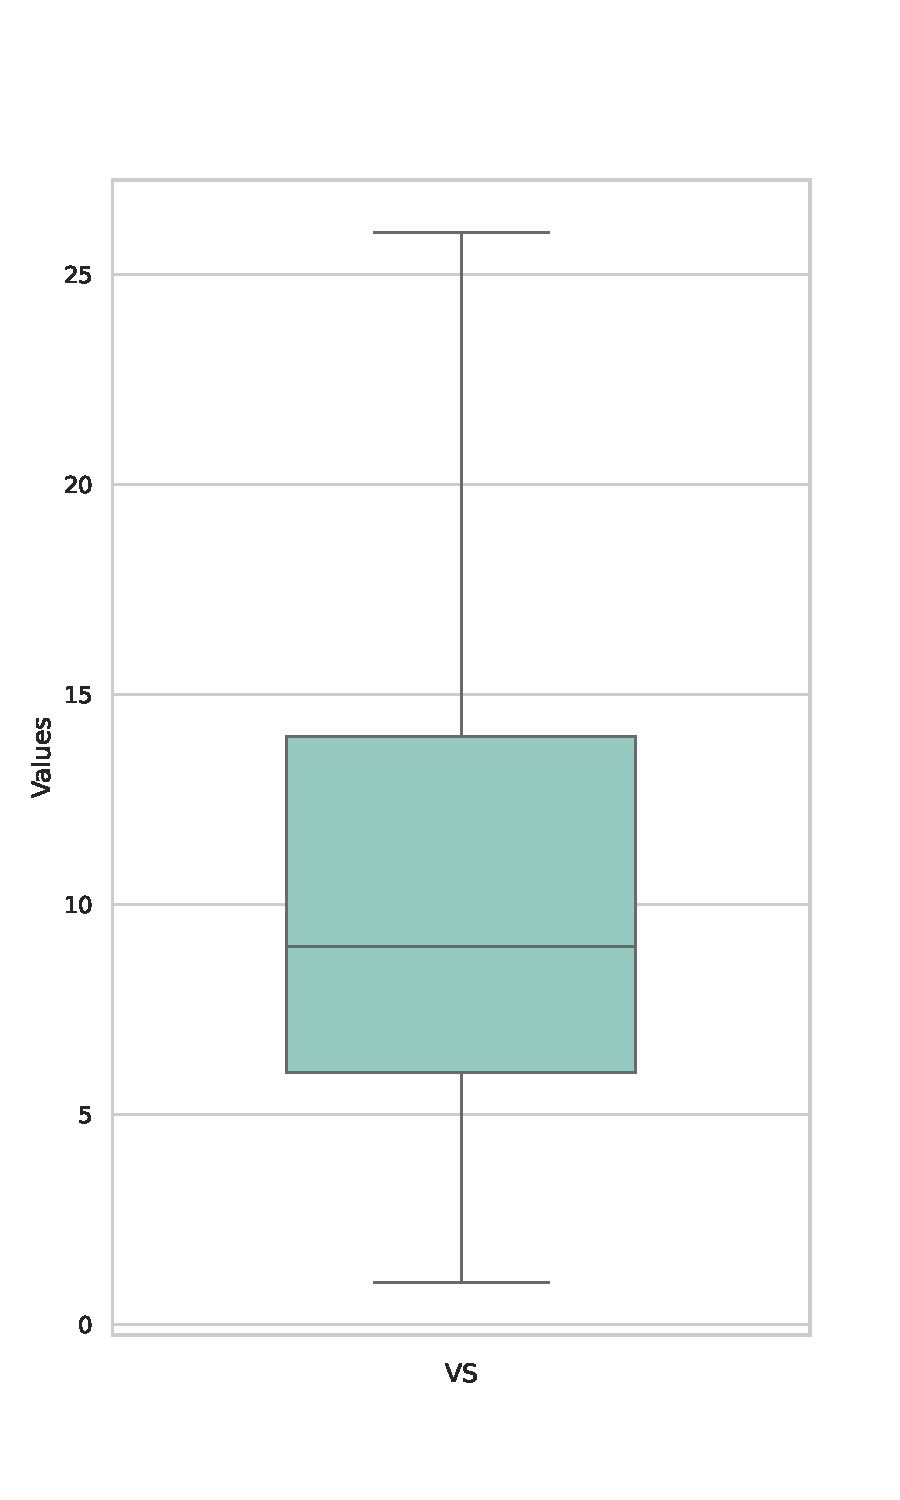
\includegraphics[width=\linewidth]{Box_Plot_of_VS.pdf}
		\caption{VS}
		\label{fig:BoxPlotVS}
	\end{subfigure}

	\vspace{1em} % Adjust vertical space between rows of images

	\begin{subfigure}[b]{\subfigwidth}
		\centering
		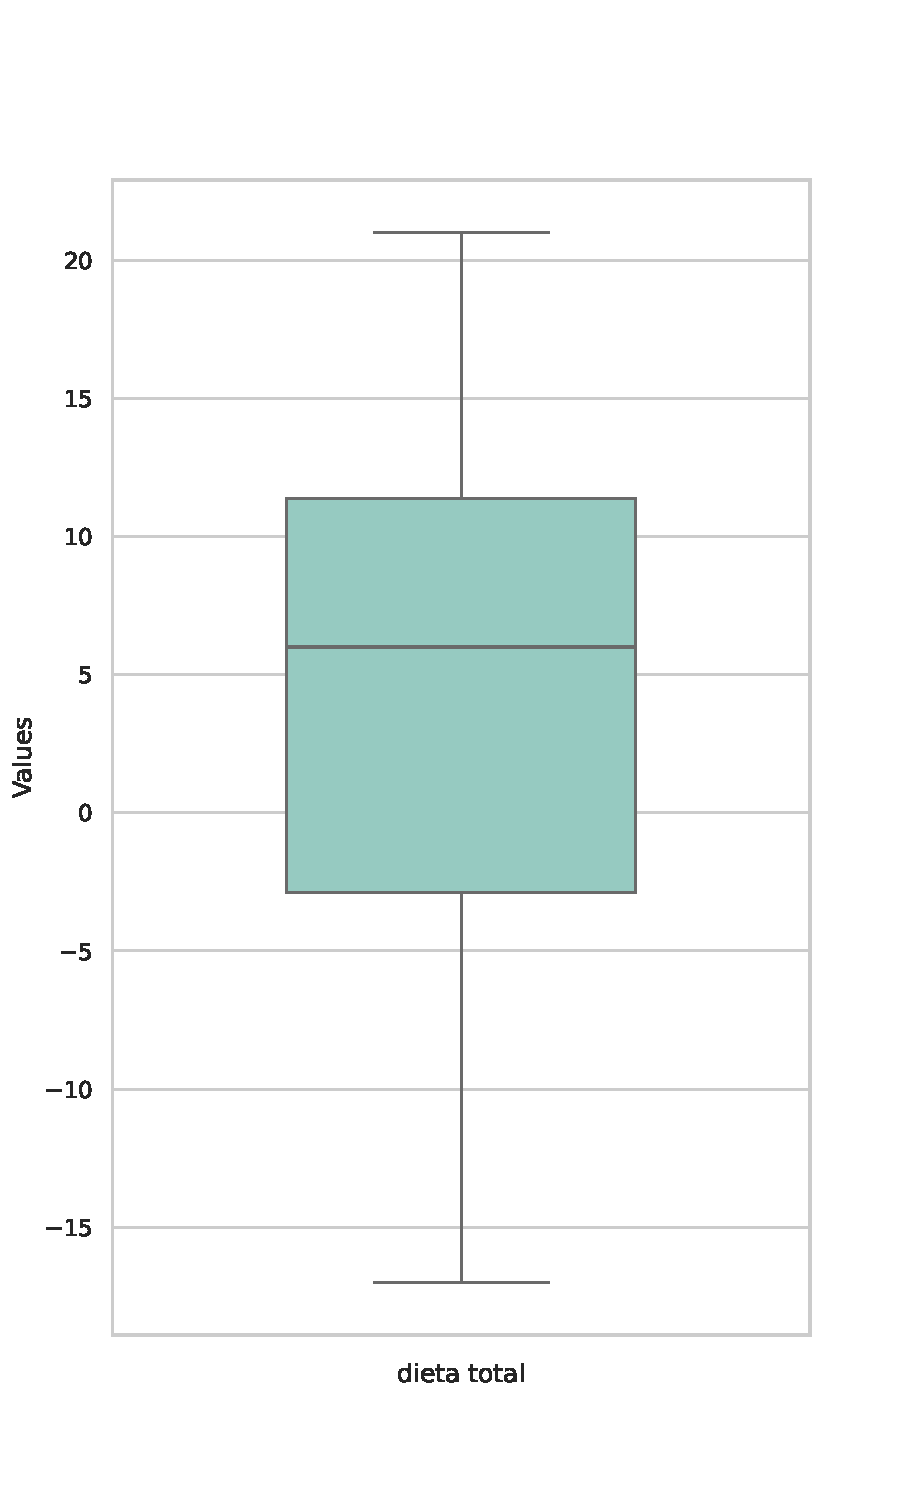
\includegraphics[width=\linewidth]{Box_Plot_of_dieta_total.pdf}
		\caption{Dieta Total}
		\label{fig:BoxPlotDietaTotal}
	\end{subfigure}
	\hspace{0.5em}
	\begin{subfigure}[b]{\subfigwidth}
		\centering
		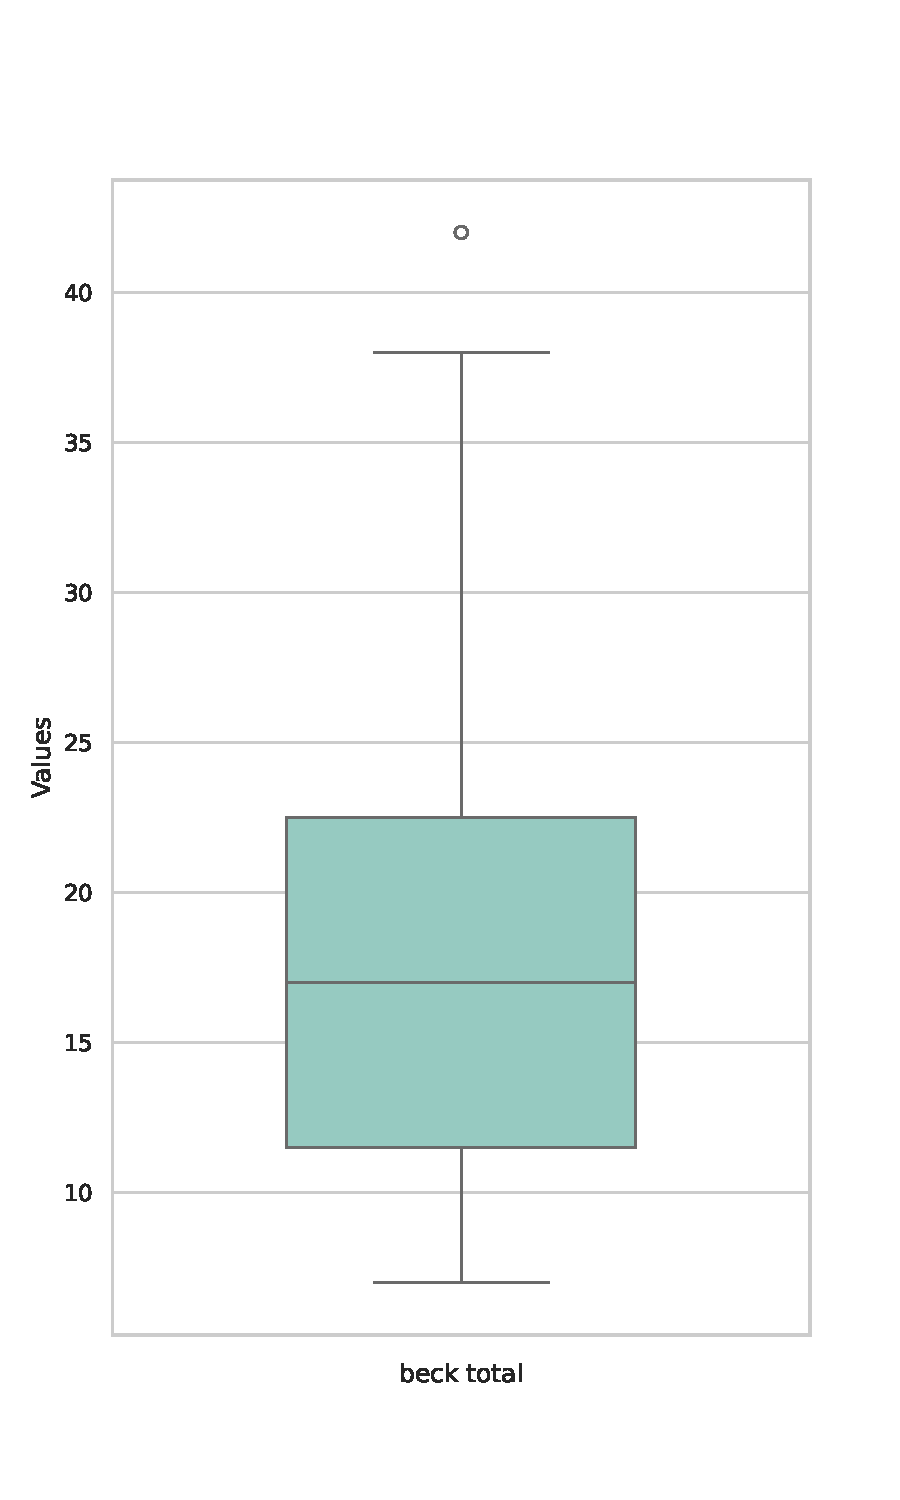
\includegraphics[width=\linewidth]{Box_Plot_of_beck_total.pdf}
		\caption{Beck Total}
		\label{fig:BoxPlotBeckTotal}
	\end{subfigure}

	\caption{Gráficos de Caja y Bigotes de las Variables}
	\label{fig:BoxPlots}
\end{figure}

	\begin{table}[]
		\resizebox{0.8\columnwidth}{!}{%
			\begin{tabular}{@{}rllrr@{}}
				\toprule
				\multicolumn{1}{l}{} & Variable \#1                  & Variable \#2               & \multicolumn{1}{l}{Correlation} & \multicolumn{1}{l}{P\_Value} \\ \midrule
				3                    & beck\_loss\_of\_pleasure     & diet\_fruit               & -0.489                          & 0.006                        \\
				7                    & beck\_suicidal\_thoughts     & diet\_fruit               & -0.480                          & 0.007                        \\
				1                    & beck\_pessimism              & diet\_sugar               & 0.432                           & 0.017                        \\
				21                   & beck\_pessimism              & age                       & -0.424                          & 0.019                        \\
				13                   & beck\_loss\_of\_interest     & diet\_soft\_drinks        & 0.418                           & 0.021                        \\
				24                   & diet\_red\_meat              & blood\_pressure           & -0.415                          & 0.022                        \\
				20                   & beck\_difficulty\_concentrating & diet\_flour            & 0.414                           & 0.023                        \\
				0                    & beck\_pessimism              & diet\_red\_meat           & 0.407                           & 0.026                        \\
				10                   & beck\_agitation              & diet\_ginger              & -0.404                          & 0.027                        \\
				2                    & beck\_failure                & diet\_olive\_oil          & 0.404                           & 0.027                        \\
				4                    & beck\_punishment             & diet\_fruit               & -0.398                          & 0.030                        \\
				8                    & beck\_crying                 & diet\_vegetables          & 0.396                           & 0.030                        \\
				6                    & beck\_dissatisfaction        & diet\_fruit               & -0.391                          & 0.033                        \\
				15                   & beck\_irritability           & diet\_red\_meat           & 0.388                           & 0.034                        \\
				16                   & beck\_irritability           & diet\_sugar               & 0.378                           & 0.039                        \\
				12                   & beck\_loss\_of\_interest     & diet\_flour               & 0.378                           & 0.040                        \\
				19                   & beck\_difficulty\_concentrating & diet\_nuts             & 0.376                           & 0.040                        \\
				17                   & beck\_irritability           & total\_diet               & -0.372                          & 0.043                        \\
				14                   & beck\_indecision             & diet\_soft\_drinks        & 0.372                           & 0.043                        \\
				25                   & diet\_flour                  & age                       & -0.367                          & 0.046                        \\
				9                    & beck\_agitation              & diet\_alcohol             & 0.366                           & 0.047                        \\
				11                   & beck\_loss\_of\_interest     & diet\_fruit               & -0.365                          & 0.047                        \\
				23                   & beck\_self\_disesteem        & age                       & -0.360                          & 0.050                        \\
				18                   & beck\_appetite\_changes      & diet\_soft\_drinks        & 0.354                           & 0.055                        \\
				22                   & beck\_indecision             & CRP (C-reactive protein)  & 0.351                           & 0.057                        \\
				5                    & beck\_punishment             & total\_diet               & -0.351                          & 0.057                        \\ \bottomrule
			\end{tabular}%
		}
		\caption{Tabla de Correlaciones}
		\label{tab:tableOfCorr}
	\end{table}




	El cuadro \ref{tab:tableOfCorr} muestra las correlaciones entre diversas variables de consumo y
	diferentes síntomas emocionales o psicológicos, junto con los valores p
	asociados que indican la significancia estadística de estas
	correlaciones.

	Existe una correlación negativa significativa entre el consumo de fruta
	y la pérdida de placer, sugiriendo que a mayor consumo de fruta, menor
	es la pérdida de placer. También existe una correlación negativa
	significativa entre el consumo de fruta y los pensamientos suicidas, lo
	que indica que a mayor consumo de fruta, menor es la frecuencia de
	pensamientos suicidas.

	Otras correlaciones que se evidenciaron fueron: una correlación positiva
	entre el consumo de azúcar y el pesimismo, sugiriendo que un mayor
	consumo de azúcar está asociado con niveles más altos de pesimismo. Una
	correlación positiva entre el consumo de gaseosas y la pérdida de
	interés, indicando que a mayor consumo de gaseosas, mayor es la pérdida
	de interés.

	Además hay una correlación positiva entre el consumo de harina y la
	dificultad de concentración, sugiriendo que un mayor consumo de harina
	está asociado con mayores dificultades para concentrarse. También hay
	una correlación positiva entre el consumo de carne roja y el pesimismo,
	indicando que a mayor consumo de carne roja, mayor es el nivel de
	pesimismo.

	Existe una correlación negativa significativa entre el consumo de fruta
	y la sensación de castigo, indicando que a mayor consumo de fruta, menor
	es la sensación de castigo. También hay una correlación negativa entre
	el consumo de fruta y la disconformidad, sugiriendo que un mayor consumo
	de fruta está asociado con menores niveles de disconformidad.

	Se observó una correlación positiva entre el consumo de carne roja y la
	irritabilidad, indicando que a mayor consumo de carne roja, mayor es la
	irritabilidad.

	La mayoría de las correlaciones negativas involucran el consumo de
	frutas, lo que podría sugerir un efecto protector del consumo de frutas
	contra ciertos síntomas psicológicos negativos. Las correlaciones
	positivas entre el consumo de azúcar y gaseosas con síntomas negativos
	como el pesimismo y la pérdida de interés podrían señalar la necesidad
	de moderar el consumo de estos productos para mejorar el bienestar
	emocional.

	Todas las correlaciones mencionadas son significativas con un valor p
	\textless{} 0.05, lo que respalda la robustez de estas asociaciones.
	Estos insights pueden ser utilizados para recomendar ajustes dietéticos
	como parte de un enfoque holístico para mejorar el bienestar emocional y
	mental.

	El $\alpha$ de Cronbach es una medida de la consistencia interna de una escala.
	Valores entre 0.7 y 0.8 generalmente se consideran aceptables,
	sugiriendo que la escala tiene una fiabilidad adecuada. En este caso, un
	valor de 0.741 indica que los ítems del cuestionario de dieta están
	razonablemente correlacionados y miden el mismo constructo subyacente.

	El $\omega$ de McDonald es otra medida de la consistencia interna y a menudo se
	considera una estimación más precisa que el $\alpha$ de Cronbach. Un valor
	superior a 0.9 se considera excelente, indicando una alta fiabilidad de
	la escala. En este caso, un valor de 0.904 sugiere que el cuestionario
	es muy confiable y que los ítems son consistentes en la medición del
	constructo.

	Ambos valores indican una buena consistencia interna, aunque el $\omega$ de
	McDonald es notablemente más alto que el $\alpha$ de Cronbach. Esto puede
	ocurrir cuando los ítems tienen diferentes cargas factoriales y el $\omega$ de
	McDonald, que toma en cuenta estas diferencias, proporciona una
	estimación más precisa de la fiabilidad. El cuestionario de dieta que
	desarrollamos es confiable para su uso en investigaciones y aplicaciones
	prácticas, dado que ambas métricas de fiabilidad superan los umbrales
	generalmente aceptados.

	\subsection{Síntomas Depresivos de Beck}
		\begin{figure}[H]
		\centering
		\includegraphicsmax{sintomasDepresivosBeckGraph.pdf}
		\caption{Mapa de Calor: Síntomas Depresivos}
		\label{fig:Figure2}
	\end{figure}
	\vspace{-1em} % Adjust vertical space

	\subsection{Hábitos Alimentarios De Las Mujeres De Jóvenes Guatemaltecas}
		\begin{figure}[H]
			\centering
			\includegraphicsmax{dietGraph.pdf}
			\caption{Mapa de Calor: Cuestionario de Dieta}
			\label{fig:Figure3}
		\end{figure}

	\section{Discusión de Resultados}\label{discusiuxf3n-de-resultados}

	Este estudio tuvo como objetivo analizar la relación entre los
	marcadores inflamatorios, la severidad de los síntomas depresivos y los
	hábitos alimenticios en mujeres jóvenes guatemaltecas. Los resultados
	obtenidos proporcionan evidencia significativa sobre estas interacciones
	y ofrecen insights valiosos para la comprensión de la relación entre
	dieta, inflamación y depresión en esta población específica.

	\subsection{Resumen de hallazgos principales}\label{resumen-de-hallazgos-principales}

	Nuestro estudio reveló correlaciones significativas entre ciertos
	patrones dietéticos y síntomas depresivos específicos. En particular, se
	encontró una fuerte asociación negativa entre el consumo de frutas y
	varios síntomas depresivos, incluyendo la pérdida de placer $(r = -0.49,
	p = 0.006)$ y los pensamientos suicidas $(r = -0.48, p = 0.007)$. Por otro
	lado, se observaron correlaciones positivas entre el consumo de
	alimentos procesados (como azúcares, gaseosas y harinas) y síntomas como
	el pesimismo, la pérdida de interés y la dificultad de concentración.\\

	En cuanto a los marcadores inflamatorios, aunque no se encontraron
	correlaciones directas significativas entre la dieta y los niveles de
	PCR y VS, se observó una tendencia que sugiere una posible relación
	entre estos factores que merece mayor investigación.


	\subsection{Interpretación de resultados}\label{interpretaciuxf3n-de-resultados}

	\subsubsection{Efecto protector del consumo de frutas}

	La correlación negativa entre el consumo de frutas y los síntomas
	depresivos sugiere un posible efecto protector de una dieta rica en
	frutas contra la depresión. Esto podría atribuirse a los nutrientes y
	antioxidantes presentes en las frutas, que pueden tener un impacto
	positivo en la salud mental. La asociación particularmente fuerte con la
	reducción de pensamientos suicidas es un hallazgo notable que merece
	mayor investigación.\\

	Esta relación podría explicarse por varios mecanismos:

	\begin{enumerate}
		\item Los antioxidantes presentes en las frutas pueden reducir el estrés
		oxidativo, que se ha asociado con la depresión.\\

		\item Las frutas son ricas en vitaminas y minerales esenciales para el
		funcionamiento neurológico óptimo.\\

		\item La fibra dietética de las frutas puede influir positivamente en la
		microbiota intestinal, que a su vez afecta el eje intestino-cerebro.
	\end{enumerate}

	\subsubsection{Impacto negativo de alimentos procesados}\label{impacto-negativo-de-alimentos-procesados}

	Las correlaciones positivas entre el consumo de alimentos procesados y
	síntomas depresivos apoyan la hipótesis de que una dieta alta en
	azúcares refinados y grasas saturadas puede contribuir al desarrollo o
	exacerbación de síntomas depresivos. Esto podría estar relacionado con
	los efectos inflamatorios de estos alimentos, aunque nuestro estudio no
	encontró correlaciones directas significativas entre la dieta y los
	marcadores inflamatorios medidos (PCR y VS).\\

	Posibles mecanismos para esta relación incluyen:

	\begin{enumerate}
		\item Los alimentos procesados pueden provocar picos de glucosa en sangre, lo que puede afectar el estado de ánimo.
		\item Estos alimentos a menudo carecen de nutrientes esenciales para la salud mental.
		\item El consumo excesivo de alimentos procesados puede llevar a la obesidad, que se ha asociado con un mayor riesgo de depresión.
	\end{enumerate}


	\subsection{Comparación con literatura existente}\label{comparaciuxf3n-con-literatura-existente}

	Nuestros hallazgos sobre el efecto protector de las frutas son
	consistentes con estudios previos que han encontrado asociaciones entre
	el consumo de frutas y verduras y un menor riesgo de depresión. Por
	ejemplo, un meta-análisis realizado por \parencite{liuFruitVegetableConsumption2016} encontró que
	un mayor consumo de frutas y verduras se asociaba con un menor riesgo de
	depresión. Sin embargo, nuestro estudio aporta evidencia específica
	sobre la relación entre el consumo de frutas y síntomas depresivos
	concretos en una población poco estudiada: mujeres jóvenes
	guatemaltecas.\\

	La asociación positiva entre alimentos procesados y síntomas depresivos también se alinea con investigaciones anteriores que han vinculado dietas occidentales (ricas en alimentos procesados) con un mayor riesgo de depresión. Por ejemplo, \parencite{laneUltraProcessedFoodConsumption2022} encontraron que una dieta caracterizada por alimentos procesados se asociaba con una mayor probabilidad de depresión y ansiedad en mujeres. No obstante, nuestro estudio proporciona una visión más detallada al examinar correlaciones con síntomas específicos. Además, se han publicado varios estudios adicionales que evalúan la relación entre el consumo de alimentos ultraprocesados y la depresión, así como otros trastornos mentales. Nuestro estudio incluyó un total de 17 estudios observacionales (n = 385,541); 15 transversales y 2 prospectivos. El mayor consumo de alimentos ultraprocesados se asoció de manera transversal con mayores probabilidades de síntomas depresivos y de ansiedad, tanto cuando estos resultados se evaluaron juntos (odds ratio de síntomas de trastornos mentales comunes: 1.53, IC95\% 1.43 a 1.63) como por separado (odds ratio de síntomas depresivos: 1.44, IC95\% 1.14 a 1.82; y, odds ratio de síntomas de ansiedad: 1.48, IC95\% 1.37 a 1.59). Además, un meta-análisis de estudios prospectivos demostró que una mayor ingesta de alimentos ultraprocesados se asoció con un mayor riesgo de depresión subsiguiente (hazard ratio: 1.22, IC95\% 1.16 a 1.28 a. Aunque encontramos evidencia de asociaciones entre el consumo de alimentos ultraprocesados y la salud mental adversa, se necesitan estudios prospectivos y experimentales rigurosamente diseñados para comprender mejor las vías causales.

	\subsection{Implicaciones}\label{implicaciones}

	Estos resultados tienen implicaciones importantes tanto para la práctica
	clínica como para la salud pública:

	\begin{enumerate}
		\item Intervenciones dietéticas: Los hallazgos sugieren que las intervenciones dietéticas, particularmente el aumento del consumo de frutas y la reducción de alimentos procesados, podrían ser estrategias efectivas para la prevención y el manejo de la depresión en mujeres jóvenes.
		\item Políticas de salud pública: Estos resultados podrían informar políticas de salud pública dirigidas a mejorar la salud mental a través de la promoción de dietas saludables. Por ejemplo, se podrían implementar programas de educación nutricional enfocados en aumentar el consumo de frutas y reducir el consumo de alimentos procesados.
		\item Enfoque integrado: La asociación entre dieta y síntomas depresivos refuerza la importancia de un enfoque integrado en el tratamiento de la depresión, que considere tanto factores psicológicos como nutricionales. Los profesionales de la salud mental podrían considerar incluir recomendaciones dietéticas como parte de sus planes de tratamiento.
		\item Prevención: Dado que nuestro estudio se centró en mujeres jóvenes, los resultados sugieren que las intervenciones dietéticas tempranas podrían tener un papel importante en la prevención de la depresión en esta población.
	\end{enumerate}


	\section{Limitaciones}\label{limitaciones}

	Es importante reconocer las limitaciones de este estudio:

	\begin{enumerate}
		\item Tamaño de la muestra: Con 30 participantes, el tamaño de la muestra es relativamente pequeño, lo que puede limitar la generalización de los resultados. Estudios futuros deberían considerar muestras más grandes para aumentar la potencia estadística.
		\item Diseño transversal: El diseño transversal del estudio no permite establecer relaciones causales entre la dieta y los síntomas depresivos. Se necesitan estudios longitudinales para determinar la dirección de la causalidad.
		\item Población específica: El estudio se centró en mujeres jóvenes guatemaltecas, lo que puede limitar la aplicabilidad de los resultados a otras poblaciones. Se necesitan estudios en diferentes grupos demográficos para confirmar si estos hallazgos son generalizables.
		\item Medidas de inflamación: Aunque se midieron la PCR y la VS, no se encontraron correlaciones significativas con la dieta o los síntomas depresivos, lo que podría deberse a la necesidad de medidas más sensibles o específicas de inflamación.
		\item Definición de patrones dietéticos: Como se ha observado en la literatura, la falta de una definición estandarizada de ``dieta saludable'' puede dificultar la comparación entre estudios. En nuestro caso, nos centramos en alimentos específicos más que en patrones dietéticos generales, lo que puede limitar la comparabilidad con otros estudios.
		\item Variabilidad en la medición de la depresión: Aunque utilizamos la escala de Beck, que es ampliamente validada, la literatura señala que la variabilidad en las medidas de depresión entre estudios puede dificultar la comparación de resultados.
		\item Factores de confusión: Aunque se controlaron varios factores demográficos y de estilo de vida, es posible que existan otros factores de confusión no medidos que puedan influir en la relación entre dieta y depresión.
	\end{enumerate}


	\section{Recomendaciones para futuras investigaciones}\label{recomendaciones-para-futuras-investigaciones}

	Basándonos en nuestros hallazgos y limitaciones, recomendamos:
	\begin{enumerate}
		\item Realizar estudios longitudinales para establecer relaciones causales entre patrones dietéticos y síntomas depresivos.
		\item Investigar los mecanismos biológicos subyacentes a la relación entre el consumo de frutas y la reducción de síntomas depresivos.
		\item Explorar la eficacia de intervenciones dietéticas específicas en la prevención y tratamiento de la depresión.
		\item Ampliar el estudio a poblaciones más diversas y de mayor tamaño.
		\item Incluir medidas más amplias y sensibles de inflamación para comprender mejor la relación entre dieta, inflamación y depresión.
		\item Estandarizar la definición y medición de patrones dietéticos para facilitar la comparación entre estudios.
		\item Utilizar múltiples medidas de depresión, incluyendo entrevistas clínicas estructuradas, para obtener una evaluación más completa de los síntomas depresivos.
		\item Investigar la interacción entre la dieta y otros factores de estilo de vida, como el ejercicio y el sueño, en relación con la depresión.
	\end{enumerate}


	\section{Conclusión}\label{conclusiuxf3n}

	Este estudio proporciona evidencia importante sobre la relación entre
	los patrones dietéticos y los síntomas depresivos en mujeres jóvenes
	guatemaltecas. Los hallazgos subrayan el potencial papel protector de
	una dieta rica en frutas y los posibles efectos negativos de los
	alimentos procesados en la salud mental. Aunque se requiere más
	investigación, estos resultados sugieren que las intervenciones
	dietéticas podrían ser un componente valioso en las estrategias de
	prevención y tratamiento de la depresión.\\

	La complejidad de la relación entre dieta, inflamación y depresión
	evidenciada en este estudio subraya la necesidad de un enfoque
	multidisciplinario en la investigación y tratamiento de la depresión. A
	medida que avanzamos en la comprensión de estas interacciones, es
	crucial que los profesionales de la salud mental, nutricionistas y
	responsables de políticas de salud pública trabajen juntos para
	desarrollar estrategias integrales que aborden tanto los aspectos
	nutricionales como psicológicos de la salud mental.


	\nocite{*}
	\printbibliography

\end{document}
%
%%%
%%% Copyright (C) 2019 by Daniel A. Weiss <daniel.weiss.led at gmail.com>
%%%
%%% This work may be distributed and/or modified under the
%%% conditions of the LaTeX Project Public License (LPPL), either
%%% version 1.3c of this license or (at your option) any later
%%% version.  The latest version of this license is in the file:
%%%
%%% http://www.latex-project.org/lppl.txt
%%%
%%% Users may freely modify these files without permission, as long as the
%%% copyright line and this statement are maintained intact.
%%%
%%% This work is not endorsed by, affiliated with, or probably even known
%%% by, the American Psychological Association.
%%%
%%% This work is "maintained" (as per LPPL maintenance status) by
%%% Daniel A. Weiss.
%%%
%%% This work consists of the file  apa7.dtx
%%% and the derived files           apa7.ins,
%%%                                 apa7.cls,
%%%                                 apa7.pdf,
%%%                                 README,
%%%                                 APA7american.txt,
%%%                                 APA7british.txt,
%%%                                 APA7dutch.txt,
%%%                                 APA7english.txt,
%%%                                 APA7german.txt,
%%%                                 APA7ngerman.txt,
%%%                                 APA7greek.txt,
%%%                                 APA7czech.txt,
%%%                                 APA7turkish.txt,
%%%                                 APA7endfloat.cfg,
%%%                                 Figure1.pdf,
%%%                                 shortsample.tex,
%%%                                 longsample.tex, and
%%%                                 bibliography.bib.
%%%
%%%
%%% End of file `./samples/longsample.tex'.